\section{The Weakly Transactional Queue} 

The Weakly Transactional Queue (FCQueueWT) demonstrates how the flat combining technique's performance is dependent upon the number of invalid histories. This queue implements a weaker transactional specification, which provides all invariants of a concurrent queue, but provides the following guarantees instead of the transactional ones listed earlier (Chapter~\ref{Queue}):
\begin{itemize}
    \item Instead of the normal pops, the queue executes \emph{LazyPops} with the following specification:
        \begin{itemize}
            \item Any two \texttt{pops} within the transaction do not need to pop consecutive values off the queue.
            \item A pop's return value \emph{cannot} be accessed during the transaction. The pops are applied and their return values determined only at commit time (hence the name LazyPop). 
        \end{itemize}
    \item A pop cannot remove an uninstalled value (i.e., a value pushed earlier in the same transaction).
    \item The \emph{atomic} property thus becomes: A transaction with multiple pops and multiple pushes guarantees that the operations will either all occur or that none will occur.
\end{itemize}

Given this specification, interleavings 1, 2, and 3 in Table~\ref{tab:interleavings} are allowable if the return value of the pop is not used within same transaction. This is because two pops in a transaction do not need to pop consecutive values off the queue. Interleaving 4 is prevented by installing all pushes in the same transaction together at commit time, and interleaving 5 is allowed because $T1$'s pop cannot see its earlier pushed value.

The queue under this specification retains all the fairness properties of a concurrent queue (no value remains in the queue forever, since values are still removed in the order in which they are added). Like Schwarz\cite{schwarz}, we see uses for this transactional queue as a buffer between producer and consumer activities, in which exact ordering of values in the buffer are unimportant.
Our specification differs from that of Schwarz\cite{schwarz}, however, by preventing a pop from seeing a push within the same transaction, and by preventing access to the return value of a pop until after the transaction commits. This allows us to utilize the flat combining approach to its full potential: we do not need to generate additional flat combining calls during transaction execution because the queue does not need to be accessed until commit time.

\subsection{Algorithm}

The FCQueueWT modifies the nontransactional, flat combining technique as follows:
   \subsubsection{Pops} 
    Executing a pop returns a LazyPop value but does not generate a flat combining request or access the queue itself. At commit time, all LazyPops are instantiated with values: for each LazyPop, the thread makes a \texttt{<POP>} flat combining request. This request is completed using the original \texttt{<POP>} flat combining implementation, which pops an item off the queue.

    \subsubsection{Pushes}
    Executing a push merely adds the value onto a \texttt{write\_list\_item}. Pushes from the same transaction are installed together, using the \texttt{<PUSH, list>} flat combining implementation from the transactional flat combining queue that takes the entire list and pushes each value onto the queue.


\subsection{Evaluation}

We evaluate the weakly transactional flat-combining queue on the same benchmarks described in Section~\ref{q_microbenchmarks} to compare against the fully transactional flat-combining queue (STO-FCQueue), the STO2 queue, and the WrappedFCQueueNT. Results are shown in Figure~\ref{lpfcqueues}.

\floatstyle{plain} 
\restylefloat{figure}
\begin{figure}[ht!]
\caption{FCQueueWT Performance}
    \centering
    \begin{tabular}{|c|c|}
        \hline&\\
        Speed (ops/s) & Aborts (\% Transactions)\\
        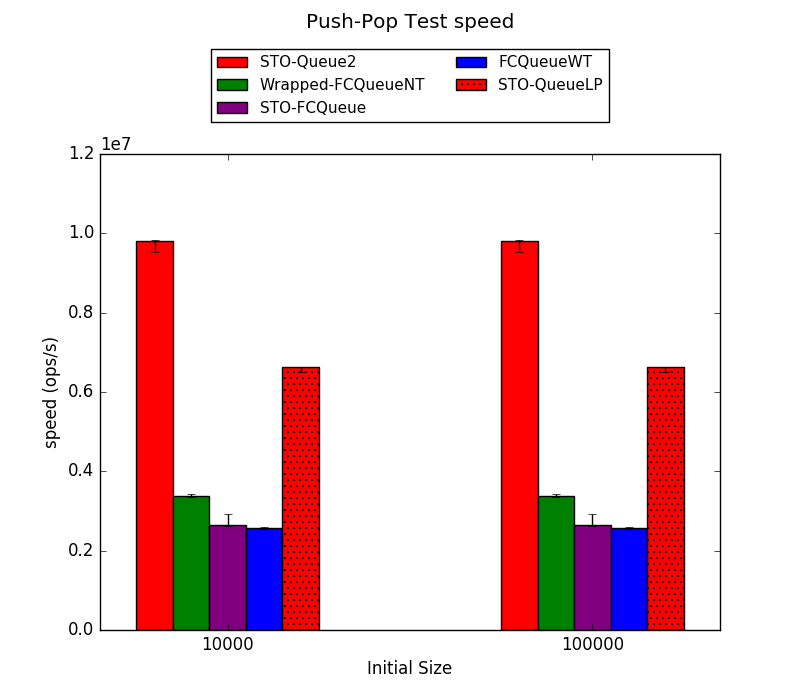
\includegraphics[height=2.25in]{fcqueues/lpQ:PushPopspeed.png} &
        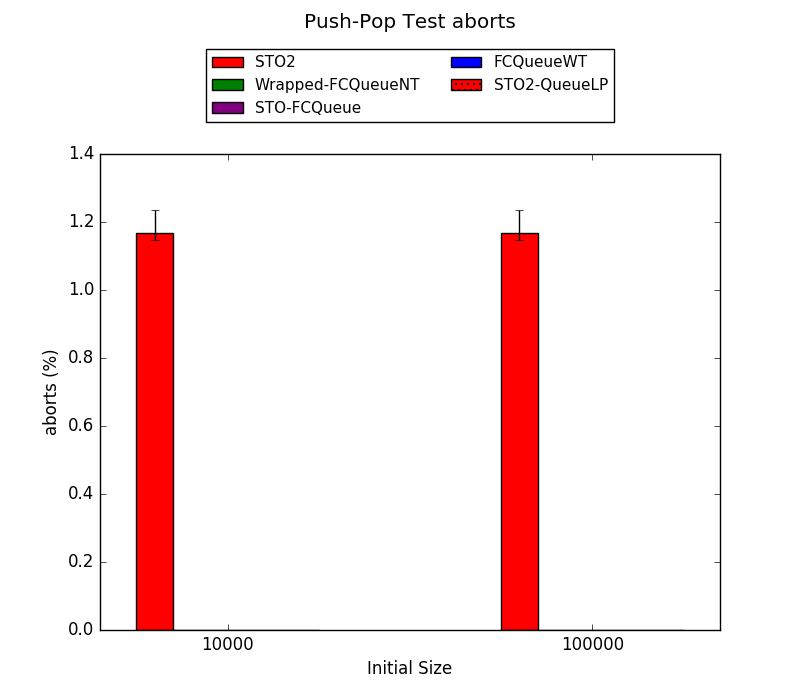
\includegraphics[height=2.25in]{fcqueues/lpQ:PushPopaborts.png}\\
        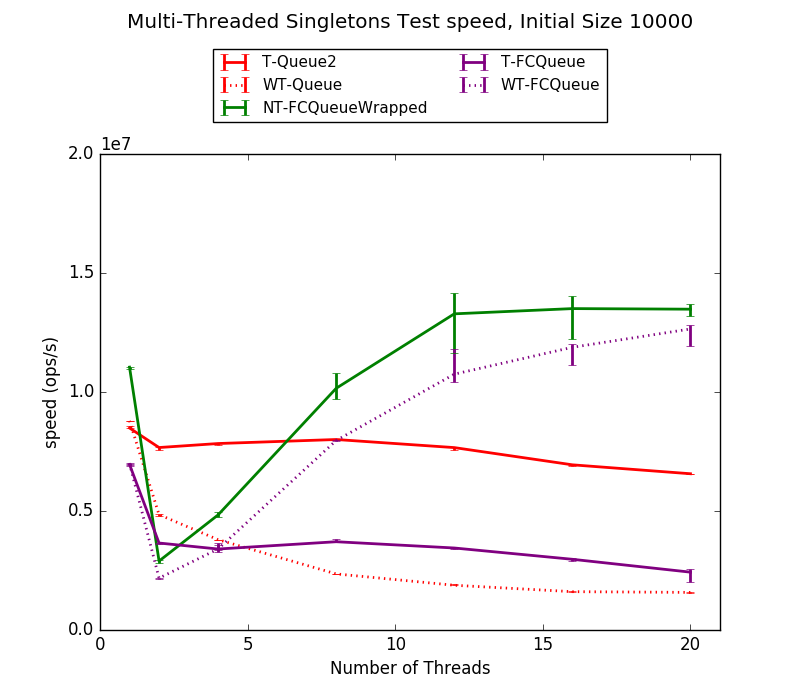
\includegraphics[height=2.25in]{fcqueues/lpQ:RandSingleOps10000speed.png} &
        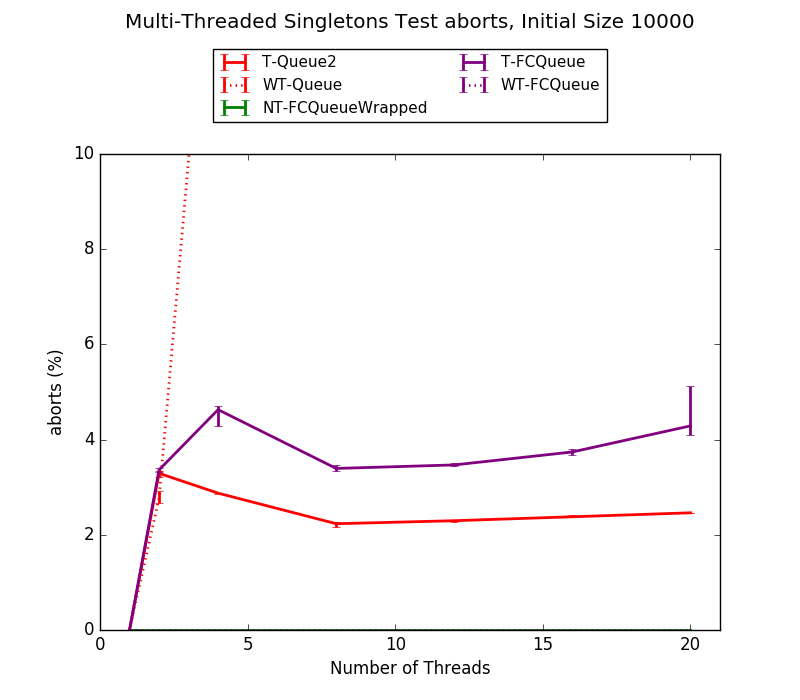
\includegraphics[height=2.25in]{fcqueues/lpQ:RandSingleOps10000aborts.png}\\
        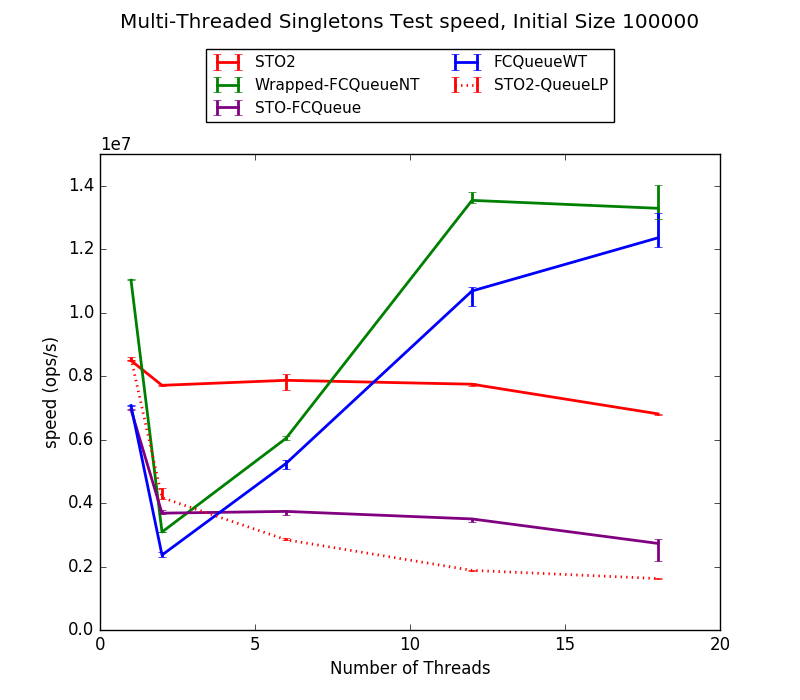
\includegraphics[height=2.25in]{fcqueues/lpQ:RandSingleOps100000speed.png} &
    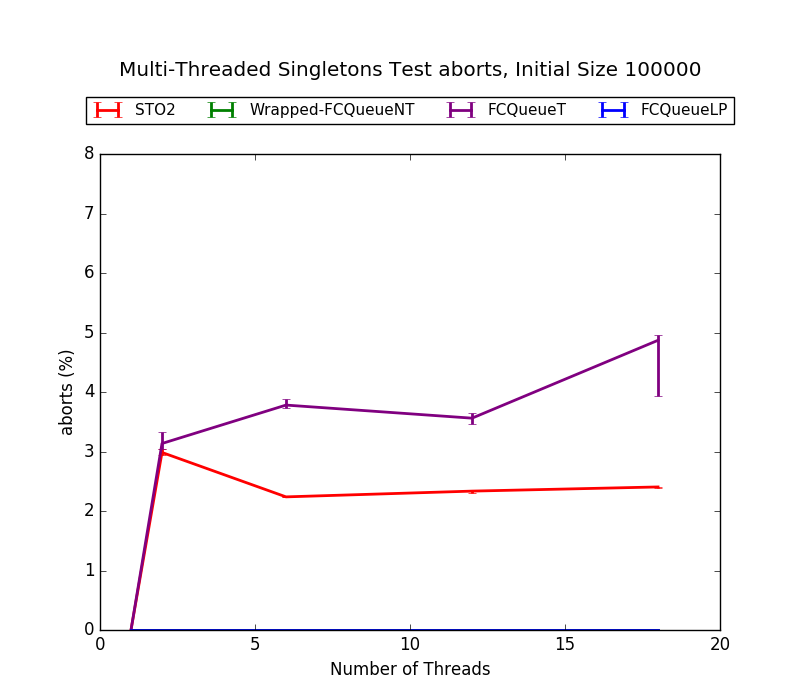
\includegraphics[height=2.25in]{fcqueues/lpQ:RandSingleOps100000aborts.png}\\
        \hline
    \end{tabular}
\label{fig:lpfcqueues}
\end{figure}

\subsection{Discussion}
While the weakly-transaction, flat combining queue does not perform as well as its nontransactional counterpart, we note that the performance exceeds that of the fully transactional STO1, STO2, and flat combining queues. In addition, FCQueueWT outperforms its STO counterpart (STO-WT), demonstrating the effectiveness of the flat combining technique in this weakly transactional setting.

\lyt{TODO ADD MORE}
